\documentclass[UTF8,10pt,twocolumn,fontset=fandol]{ctexart}

\usepackage[letterpaper,margin=0.72in,columnsep=0.22in]{geometry}
\usepackage{amsmath,amssymb,mathtools}
\usepackage{booktabs,array,multirow}
\usepackage{graphicx}
\usepackage[dvipsnames]{xcolor}
\usepackage{tikz}
\usetikzlibrary{arrows.meta,positioning,fit,calc,shapes.geometric,backgrounds}
\usepackage{enumitem}
\usepackage{microtype}
\usepackage{url}
\usepackage[colorlinks=true,allcolors=MidnightBlue,unicode=true]{hyperref}
\hypersetup{
    pdftitle={TopoContour-Mamba：基于增广等高线树的拓扑引导视觉序列化},
    pdfauthor={Dian Yu and Haoyu Yang},
    pdfsubject={基于增广等高线树的显著性有序视觉状态空间建模},
    pdfkeywords={Vision Mamba, 状态空间模型, 视觉显著性, 增广等高线树, 视觉序列化, 扫描顺序}
}

\setlist{nosep,leftmargin=*}
\setlength{\emergencystretch}{2em}
\newcommand{\method}{TopoContour-Mamba}
\newcommand{\NormalM}{\mathcal{M}_{\mathrm{N}}}
\newcommand{\ContourM}{\mathcal{M}_{\mathrm{C}}}
\newcommand{\MergeM}{\mathcal{M}_{\mathrm{G}}}
\newcommand{\Gate}{\mathcal{G}}
\newcounter{algorithm}

\title{\textbf{TopoContour-Mamba：\\基于增广等高线树的拓扑引导视觉序列化}}
\author{Dian Yu \and Haoyu Yang}
\date{}

\begin{document}
\maketitle

\begin{abstract}
视觉状态空间模型必须先把图像排成序列，再执行选择性扫描，因此路线决定哪些信息先进入历史、哪些信息靠近最终读出。多数视觉路线对所有图像固定。本文提出\method：用确定性显著性场为每张图像生成路线，再沿路线直接读取原图像素。完整等高线树提供延续、分裂、汇合、源点和终止关系；只有值得扫描的常规轮廓才插入稀疏执行树。每个保留轮廓先按周长确定点数，再由均匀试探点读取同一张Sobel场：法线方向响应的平均符号为整圈选择低显著性普通读取侧，平滑后的响应强度重分配固定点数，最大强度位置确定共同起止点 $p_0$。Normal Mamba从首次碰撞点读回带Tag的轮廓点。两次共享参数的Contour Mamba扫描从 $p_0$ 出发，按相反方向遍历同一组闭环点，并在带Tag的 $p_0$ 副本结束。每条树枝的终止圈读取两侧法线，再用第二对闭环汇集。所有轮廓独立编码完成后，Tree Mamba才从低显著性向高显著性汇总带Tag输出：分裂复制摘要，汇合采用与输入顺序无关、考虑采样支撑量的融合。最后，各终止叶按实际读取区域的显著性排序，并由最终Mamba完成分类。初版路线完全确定，不使用CNN特征Stem。本文完整规定路线、Token接口、边界情况、默认值和结构性质，不作实证性能声明。
\end{abstract}

\section{引言}

Mamba通过输入相关的状态更新实现线性序列建模，但扫描前仍然需要确定Token顺序 \cite{gu2023mamba}。Vision Mamba通常采用栅格、方向、窗口或其他预先设计的路线 \cite{zhu2024vim,liu2024vmamba,yang2024plainmamba,huang2024localmamba}。这些路线便于并行计算，却不一定符合当前图像自身的结构。

本文的直觉很简单。人观察图像时，不会对所有区域投入相同精度：宽泛背景可以先获得粗略认识，醒目的局部细节则得到更晚、更密集的读取。本文不声称模拟生物视觉，只把这一想法用于安排选择性状态空间模型的信息顺序。低显著性信息较早进入全局历史，高显著性信息较晚进入；热力变化快的位置获得更密的采样。每次Mamba扫描开始前，完整顺序都已经确定。

\method{}从显著性标量场生成这个顺序。闭合等值线分量形成局部路线，等高线树记录这些分量随显著性升高而出现、延续、分裂、汇合和终止的关系 \cite{carr2003contourtrees}。因此不需要把每个圈强制匹配到最近的下一层圈，也不会在盆地周围产生错误的远距离连接。细小树枝可以保留在拓扑中，但不一定消耗扫描Token。

初版使用传统算法生成显著性场，并直接从原始RGB图像读取视觉内容，不包含CNN特征Stem。同一张Sobel场统一完成三个决定：带符号的法线响应为整圈选择低显著性读取侧，响应强度决定圈内采样密度，最强的平滑响应位置确定公共锚点 $p_0$。这样不再为方向、密度和起止点分别设计互不相关的规则。

局部读取与全局汇总严格分开。每个保留轮廓独立编码：Normal Mamba从碰撞点读回带Tag的轮廓点；两条Contour Mamba从同一个 $p_0$ 出发，按相反方向绕圈，并在带Tag的 $p_0$ 副本结束。每条树枝的终止圈读取两侧法线，再进行第二次闭环汇集。所有局部编码完成后，Tree Mamba才沿稀疏增广等高线树从低到高处理轮廓摘要。图~\ref{fig:local}展示按照这些规则生成的一条完整路线。

本文贡献可概括为：
\begin{itemize}
    \item 用闭合等值线与低到高的增广等高线树构造随输入变化的视觉序列；
    \item 用一套Sobel规则统一决定整圈读取侧、固定预算内的采样密度和公共锚点；
    \item 用带Tag的原图像素法线与闭环编码器完成局部读取，再以Tree Mamba处理分裂、无序汇合、终止叶和空路线。
\end{itemize}

本文给出完整的架构与算法规范。其贡献是确定性路线构建、Token接口、拓扑汇总规则和结构分析；本文不作实证性能声明。

\section{相关工作}

\subsection{视觉状态空间模型的序列化}

选择性状态空间模型接收有序序列，因此视觉模型必须同时决定空间邻接与读出方向。Vim把图像Patch展平，并结合位置编码使用双向状态空间块 \cite{zhu2024vim}。VMamba的SS2D沿四条路线遍历特征网格，在保持稠密网格覆盖的同时组合多方向上下文 \cite{liu2024vmamba}。PlainMamba用连续二维路线改善相邻Token的空间连续性，并加入方向感知更新 \cite{yang2024plainmamba}。LocalMamba把网格分成局部窗口，并为不同网络层搜索合适的扫描选择，以加强短程二维依赖 \cite{huang2024localmamba}。这些方法逐步改善了空间邻接，但基本几何单元仍是行列、连续网格路径或窗口，并不来自当前图像等值线的连通结构。

后续工作开始让路线随内容变化。DAMamba通过Dynamic Adaptive Scan学习扫描顺序和区域 \cite{li2025damamba}。QuadMamba预测Token局部性并递归划分窗口象限，以Gumbel-Softmax掩码和直通估计器训练离散分区 \cite{xie2024quadmamba}。面向视频超分辨率的MambaVSR构建语义连通图、聚类相关内容，再沿所得空间顺序交织时域特征 \cite{he2025mambavsr}。它们与\method{}一样反对所有图像共享单一栅格顺序，但所组织的对象不同：前述方法调整排列、区域、象限或语义组；本文提取闭合等值线分量，并在等高线树中显式保留其分裂与汇合演化。初版路线是确定性的，因此这里只主张架构差异，不声称适应性更强。

PRISMamba是最接近的几何对照。它把图像划分为同心环，在每个环内做与次序无关的聚合，再用短径向SSM在环之间传递上下文 \cite{hsieh2026prismamba}。\method{}不假设统一中心或同心圆结构：同一层可以有多个不相连、非凸的轮廓，每圈沿弧长双向扫描；法线负责读取邻带，独立的等高线树负责全局低到高汇总。因此，PRISMamba按图像中心组织稠密环，而本文按标量拓扑组织稀疏、随输入变化的等高线。

\begin{center}
\refstepcounter{table}\label{tab:comparison}
\begin{minipage}{\columnwidth}
\small\textbf{表 \thetable：}代表性视觉序列化规则。比较对象是路线结构，而不是Mamba门控本身。

\vspace{2pt}
\fontsize{7.3pt}{8.0pt}\selectfont
\setlength{\tabcolsep}{2pt}
\begin{tabular}{@{}>{\raggedright\arraybackslash}p{0.21\columnwidth}>{\raggedright\arraybackslash}p{0.25\columnwidth}>{\raggedright\arraybackslash}p{0.44\columnwidth}@{}}
\toprule
方法 & 路线 & 与本文的关键区别 \\
\midrule
Vim / VMamba & Patch/网格方向 & 稠密坐标路线，不提取等值线拓扑 \\
Plain-/\\LocalMamba & 连续路径或窗口 & 在预设网格单元内改善连续性或局部性 \\
DAMamba / QuadMamba & 学习顺序、区域或象限 & 可训练空间组织，但无显式等高线树 \\
MambaVSR & 语义分组与图顺序 & 面向复原的内容路线，而非标量等值集 \\
PRISMamba & 同心环、\\径向SSM & 统一中心，不描述分裂与汇合演化 \\
本文 & 法线、闭合轮廓与树 & 分离邻带读取、圈内编码和拓扑汇总 \\
\bottomrule
\end{tabular}
\end{minipage}
\end{center}

\subsection{显著性、轮廓与拓扑结构}

经典视觉注意模型组合亮度、颜色与方向线索，频率调谐显著性则在Lab空间测量对比度 \cite{itti1998saliency,achanta2009frequency}。这类热力图表示自底向上的醒目程度，不保证等同于任务语义重要性。本文初版使用频率调谐方法，只为序列化实验提供可复现的标量场；任务相关CNN将在第~\ref{sec:future}节讨论。由于硬轮廓提取是离散过程，必须明确其梯度边界。

等高线树记录标量阈值变化时，等值线连通分量如何出现、延续、分裂、汇合和消失 \cite{carr2003contourtrees}。增广操作把常规轮廓或网格元素关联到树弧，按需增广可避免生成不需要的几何对象 \cite{sharma2018augmentation,gueunet2019augmented}。已有神经网络工作把等高线树层次或拓扑图用于分割 \cite{he2020contourtreegnn,adame2025topovmunet}。本文既不预测等高线树，也不只把它作为损失；它是确定性执行图：常规轮廓定义相互独立的局部Mamba序列，只有完成后的带Tag输出在树上传递。

Graph Mamba处理任意图邻域的排序和状态空间编码 \cite{behrouz2024graphmamba}。本文使用的图更窄，也更受约束：标量值天然给每条树边低到高的方向，分裂与汇合语义已知，未采样路径可收缩而无需虚构最近邻连接。因此可以为不同事件使用专门算子——分裂复制、汇合无序融合、非分叉树段运行Mamba——而不是套用统一的通用图Token规则。

\paragraph{本文定位。}
创新点并非孤立地“换一条曲线”，而是把现有扫描设计常混在一起的三种关系分开：首次碰撞法线决定局部跨层证据，闭合等高线决定分量内部顺序，增广等高线树决定全局信息走向。表~\ref{tab:comparison}陈述这些架构差异；本文贡献属于方法层面，不是实证优势声明。

\section{路线构建}
\label{sec:route}

\subsection{显著性场与稀疏增广树}

设归一化原始RGB图像为 $I\in[0,1]^{H\times W\times3}$。确定性算法生成显著性场 $S\in[0,1]^{H_r\times W_r}$。默认使用频率调谐Lab对比度 \cite{achanta2009frequency}，随后进行高斯平滑。模型从 $I$ 读取RGB；$S$ 只负责构建路线并提供路线属性。

在路线网格外增加一圈低于场值范围的边框，使接触图像边缘的轮廓闭合。每个网格单元固定按西北到东南的对角线剖分，相同标量值使用确定性的符号微扰。保留扫描层级之前，先在完整分片线性场上建立等高线树 $T$。补边后的矩形单连通，因此 $T$ 无环。树可以同时包含分裂和汇合鞍点，但同一次分裂产生的兄弟支路不会再次汇合；汇合只组合具有独立低值来源的分支。有孔洞的定义域需要改用Reeb图。

在 $L$ 个常规层级提取闭合轮廓，删除低于周长和面积阈值的小圈，并把其余轮廓插入对应树弧。没有保留轮廓的路径被收缩，得到稀疏执行树 $T_A$。这样，树负责跨层拓扑，细小分支不必消耗Token；法线碰到哪个对象都不会改变树边。

热力图平滑后，在路线网格上只计算一次 $3\times3$ Sobel场 $G=(G_x,G_y)$。所有轮廓共享这张场。

\subsection{统一的Sobel方向、密度与锚点}

对周长为 $P_C$ 的保留轮廓 $C$，先确定唯一点数：
\begin{equation}
N_C=\max\!\left(N_{\min},\operatorname{round}(P_C/\delta_0)\right).
\label{eq:budget-zh}
\end{equation}
默认 $N_{\min}=16,\delta_0=2$。点数没有语义上的最大值；长圈进入更大的长度桶，或者使用不丢点的精确分块扫描。变密度操作只能移动固定数量的点，不能让某个局部额外产生Token。

先把轮廓统一定向为顺时针，再沿弧长均匀放置 $M_C=2N_C$ 个试探点。设试探点为 $u_i$，按照统一环绕方向确定的单位法线为 $n_i$。在Sobel场中双线性读取后，得到一个带符号的法线响应：
\begin{equation}
r_i=G(u_i)^{\top}n_i.
\label{eq:sobel-response-zh}
\end{equation}
它的符号表示哪一侧热力值升高。若所有 $r_i$ 的平均值不小于零，说明正法线整体指向高值侧，整圈普通法线统一选择负法线侧；否则统一选择正法线侧。平均值恰为零时固定选择负法线侧。每个圈只作一次方向判断，不允许采样点各自改变左右方向。

绝对强度 $g_i=|r_i|$ 表示热力图跨越轮廓时变化得多快。沿闭环用 $(1,2,3,2,1)/9$ 平滑一次，得到 $\bar g_i$。令 $m_C$ 为正值 $\bar g_i$ 的中位数；如果整圈没有正响应，则全部密度权重设为1。否则：
\begin{equation}
w_i=\operatorname{clip}\!\left(\frac{\bar g_i}{m_C+\epsilon},1,3\right).
\label{eq:density-zh}
\end{equation}
弱变化区域保持基础密度，强变化区域获得更多点，最大权重限制避免小区域耗尽点数预算。当标量层级间隔固定时，较大的法线方向梯度也近似表示相邻等高线距离更短。

在尚未截断的平滑强度 $\bar g_i$ 中选择最大值所在试探点作为锚点 $p_0$；并列时选择图像坐标 $(y,x)$ 字典序最小的点。因此，同一批Sobel测量同时确定读取侧、采样密度和起止点，试探阶段不需要碰撞查询。

对每个试探区间，把实际弧长乘以两端平均权重，得到加权弧长。以 $p_0$ 为起点，在累计加权弧长上等间隔放置恰好 $N_C$ 个最终点，并强制保留 $p_0$。高权重区间的点更近，但总点数不变。整个过程不拉伸、不截断，也不补造几何点。顺、逆时针扫描使用同一组物理点的相反顺序。

只有重采样结束后才进行射线碰撞查询。每个最终点向整圈选定的普通侧发射射线，直到首次正向碰到其他保留轮廓折线或补边框；忽略起点接触和本轮廓的两条相邻线段。终止圈还会向相反侧发射第二条射线。路线坐标映射回原图后，RGB与显著性都用双线性插值读取。试探点本身不成为模型Token。

\begin{figure*}[t]
    \centering
    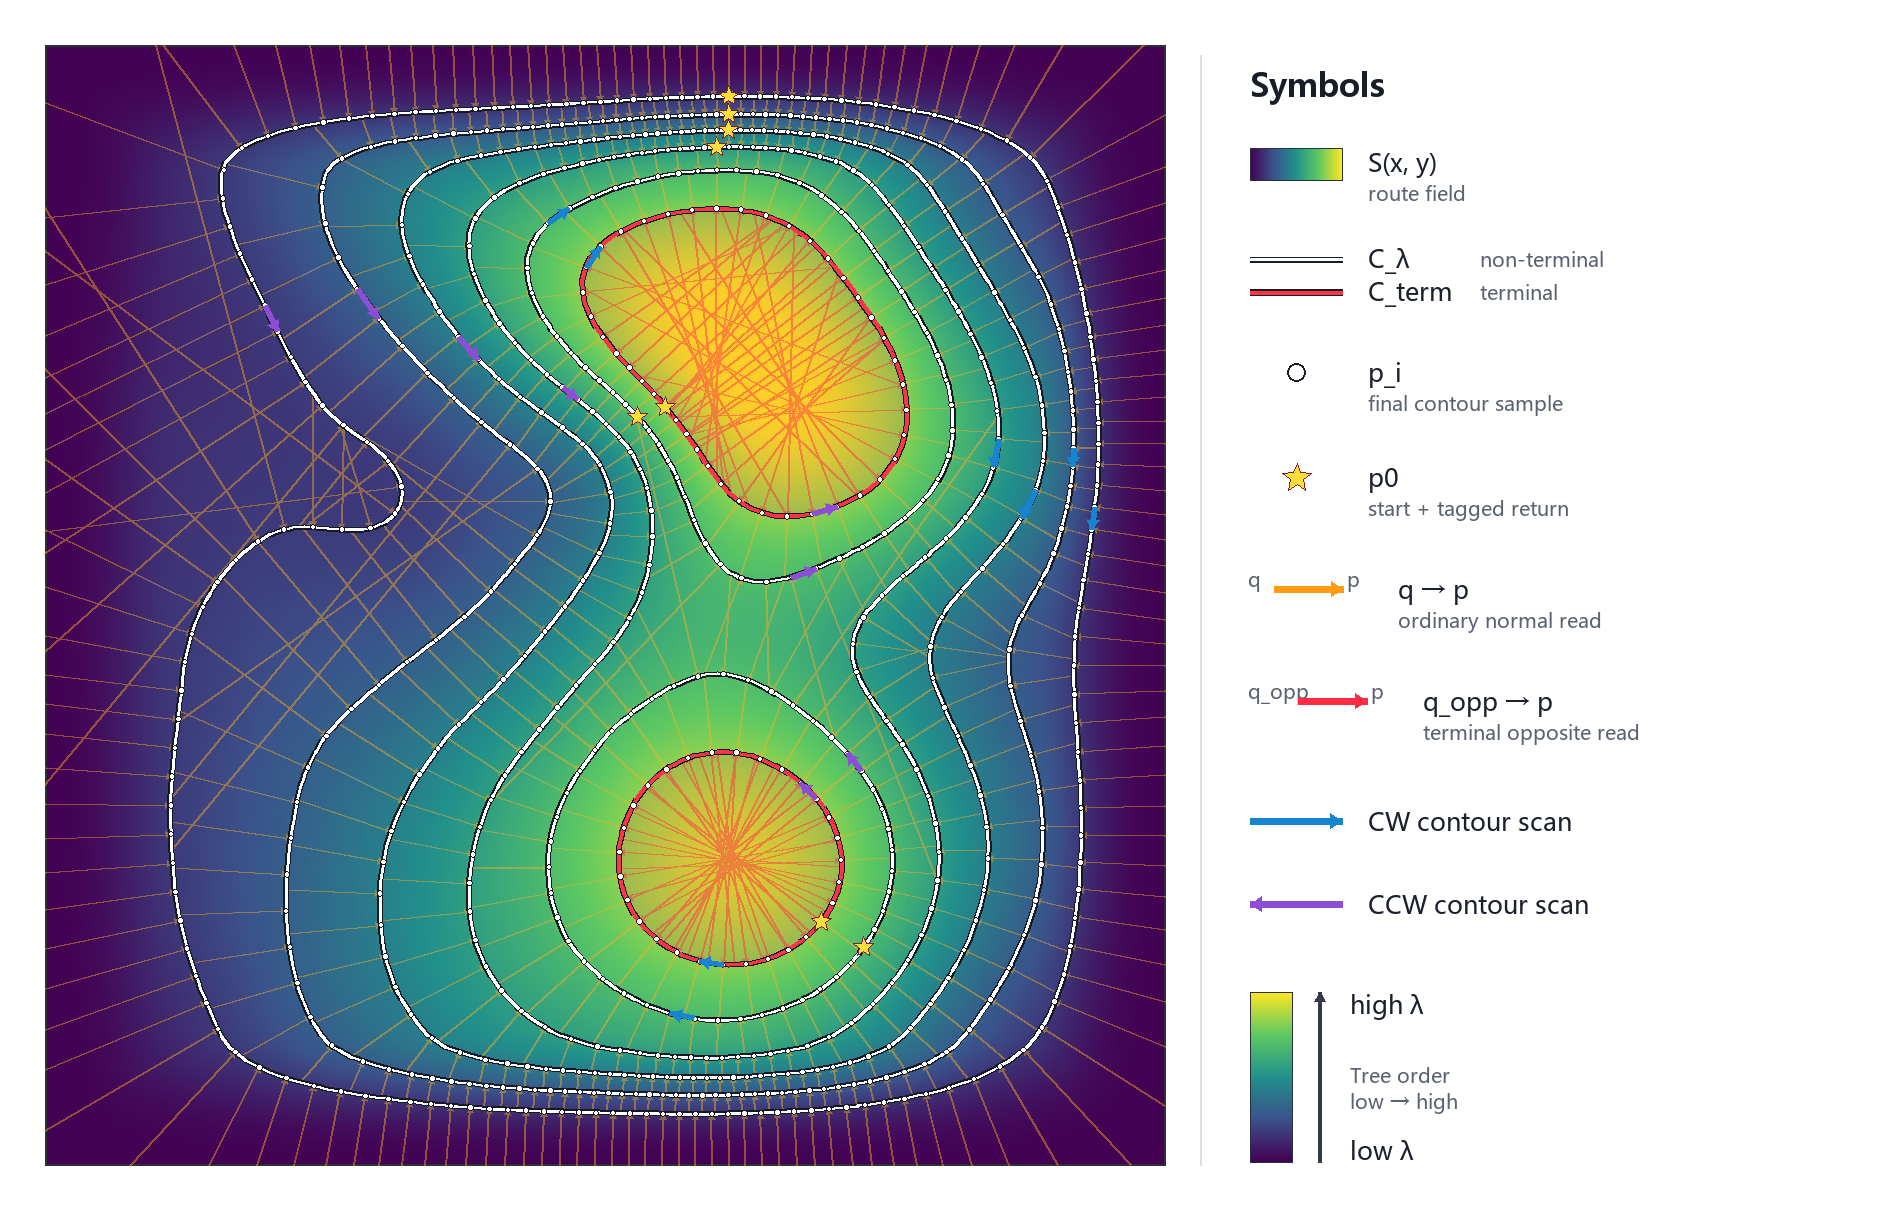
\includegraphics[width=0.84\textwidth]{figures/topocontour_paper_figure.png}
    \caption{按照本文规则生成的一条实际路线。白线表示保留的非终止轮廓；红线及浅红区域表示每条可见树枝最后保留的终止圈。橙色箭头表示Normal Mamba从首次碰撞点 $q$ 读回轮廓点 $p$ 的普通侧法线；红色箭头表示仅在终止圈补读的相反侧法线。星号表示共同起点和带Tag返回点 $p_0$，蓝色与紫色箭头表示两个闭环方向。}
    \label{fig:local}
    \vspace{0.35em}
    \begin{minipage}{0.84\textwidth}
    \small\textbf{设计哲学。}
    这条路线并不把低显著性区域判定为无用信息，也不删除它们。宽泛背景先进入历史；Sobel变化较弱的地方采样相对稀疏，而轮廓变化明显、位于树枝终点的证据后进入并更靠近带Tag的读出。因此，选择性遗忘在这里被用作一种注意力调度：较弱背景可以逐渐变模糊但仍然存在，辨识度较高的证据则较少受到后续更新影响。这只是归纳偏置，并不保证Mamba无损记忆。由于几何路线在扫描前已经确定，而且各轮廓的局部编码互相独立，图像相关的顺序仍可保持法线之间和轮廓之间的并行执行。
    \end{minipage}
\end{figure*}

\section{架构}
\label{sec:architecture}

\subsection{直接读取原图的法线与轮廓编码}

所有保留轮廓独立编码。任何父圈输出都不进入法线或闭环扫描。这是局部视觉读取与全局树汇总之间的明确分界。

考虑层级为 $\lambda_C$ 的最终轮廓点 $p$。路线构建已经为整圈固定普通读取侧 $\sigma_C$。从 $p$ 向该侧发射射线，首次碰撞为 $q_p$。几何查询从 $p$ 找到 $q_p$，但Normal Mamba按相反方向读取，也就是从 $q_p$ 回到 $p$。

对法线采样位置 $r$，记双线性读取的归一化RGB为 $c(r)$。输入还包含归一化图像坐标、$(\lambda_C,S(r)-\lambda_C)$、从碰撞点到轮廓点的相对进度，以及法线实际长度。共享逐点投影 $E_N$ 把这些值映射到模型宽度；它不是CNN，也不会混合相邻图像位置。最后的轮廓点 $p$ 加入法线终点Tag：
\begin{equation}
n_p=\NormalM\!\left(E_N[c,S-\lambda_C,\lambda_C,\hat x,\hat y,t,d]_{q_p\rightarrow p}
+e_{\mathrm{N,end}}@p\right)_p.
\label{eq:normal-zh}
\end{equation}
带Tag输出 $n_p$ 是该条原图RGB法线序列的摘要。

构造轮廓点Token时，仍直接加入端点RGB，而不要求 $n_p$ 无损保存它。共享投影 $E_C$ 把 $n_p$、$c(p)$、归一化坐标、$\lambda_C$、当前点代表的局部弧长，以及法线方向和长度组合成 $x_p$。坐标告诉Mamba点在二维图像中的位置；局部弧长则说明变密度采样后相邻Token的真实间距。

设最终点为 $(p_0,\ldots,p_{N_C-1})$，其中 $p_0$ 是重采样时保留的Sobel锚点。闭合曲线没有天然起点，因此只在序列层面从 $p_0$ 切开，几何上仍保持闭环。两个方向都从不带轮廓终点Tag的 $p_0$ 开始。顺时针依次访问 $p_1$ 到 $p_{N_C-1}$；逆时针按相反顺序访问同一组点。最后都回到第二个 $p_0$，只有返回副本带轮廓终点Tag：
\begin{align}
X_C^{\circlearrowright}&=(x_{p_0},x_{p_1},\ldots,x_{p_{N_C-1}},x_{p_0}+e_{\mathrm{C,end}}),\\
X_C^{\circlearrowleft}&=(x_{p_0},x_{p_{N_C-1}},\ldots,x_{p_1},x_{p_0}+e_{\mathrm{C,end}}).
\end{align}
每个非锚点在每个方向中出现一次；锚点分别作为不带Tag的开头和带Tag的结尾。两个带Tag返回位置的输出经拼接、投影和归一化得到局部轮廓Token $y_C$。Tag只固定读出位置，不保证无损记住全圈。终止圈还会保留两方向对齐后的逐点输出。

\paragraph{终止圈的双侧读取。}
若 $C$ 没有更高的有效后继，它就是该树枝最后一个保留圈。此时，普通侧法线和第一对闭环已经完成。每个点再向 $\sigma_C$ 的相反侧寻找首次碰撞，第二侧Normal Mamba同样从碰撞点读回带Tag的轮廓点 $p$。

在每个 $p$ 上，把第二侧法线输出与第一次顺、逆时针闭环在该点的对齐输出融合。第一次闭环输出中已经包含普通侧法线信息。融合后的点再由同一Contour Mamba执行第二对闭环，继续使用同一个 $p_0$、同一组采样点、相反的环绕顺序和带Tag的返回终点。两个最终输出融合为 $y_C^{\mathrm{term}}$。因此终止结果同时包含两侧法线，而不是用另一侧替换普通侧。峰点、宽峰环和盆地边界都使用同一规则，不需要判断是否填充内部。

法线、普通闭环和终止闭环都按真实长度分桶。填充位置放在真实带Tag终点之后并被屏蔽，读出始终索引真实终点。

\subsection{Tree Mamba汇总}

所有局部Token产生后，才从低到高处理 $T_A$。最大非分叉树段 $B$ 包含按标量值排列的轮廓 $(C_1,\ldots,C_r)$。共享Tree Mamba接收入口摘要和局部轮廓Token：
\begin{equation}
b_B=\MergeM\!\left(y_B^{\mathrm{in}},y_{C_1},\ldots,y_{C_r}+e_{\mathrm{seg}}\right)_r.
\label{eq:branch-zh}
\end{equation}
终止圈在树段中使用 $y_C^{\mathrm{term}}$ 替换第一次的 $y_C$。树源使用可学习入口Token。最后一个真实轮廓带树段终点Tag；若它也是拓扑叶子，再加叶子Tag。跨树段只传递带Tag输出 $y$，不传隐藏状态、卷积缓存或其他循环状态。

分裂鞍点把 $b_B$ 复制给各条输出树段。同一次分裂产生的兄弟支路不会在等高线树中再次汇合，因此不需要循环协调规则。

汇合鞍点的输入来自不同低值源，没有天然顺序。设第 $i$ 条分支摘要为 $b_i$，其历史代表的唯一最终轮廓采样点数为 $Q_i$。采用考虑支撑量且与输入排列无关的融合：
\begin{align}
s_i&=\tfrac12\log(1+Q_i)+\Gate(\operatorname{LN}(b_i)),\\
\alpha_i&=\frac{\exp(s_i)}{\sum_j\exp(s_j)},\qquad
b_{\mathrm{join}}=\operatorname{LN}\!\left(W_J\sum_i\alpha_i b_i+e_{\mathrm{join}}\right).
\label{eq:join-zh}
\end{align}
$\Gate$ 的末层采用零初始化，因此开始时近似按采样支撑量的平方根加权，之后再学习内容修正；整个过程不依赖不稳定的 $\|y\|$。同一算子适用于任意汇合度。

\begin{figure}[t]
    \centering
    \begin{tikzpicture}[font=\scriptsize,scale=0.82,
    node/.style={circle,draw=MidnightBlue,fill=Blue!7,minimum size=0.52cm,inner sep=0pt},
    event/.style={diamond,draw=BrickRed,fill=Red!8,minimum size=0.62cm,inner sep=0pt},
    arr/.style={-{Latex[length=1.6mm]},thick,draw=black!70}]
\node[node] (s0) at (0,0) {$b_0$};
\node[event] (split) at (0,-0.86) {S};
\node[node] (a) at (-0.92,-1.78) {$b_a$};
\node[node] (b) at (0.92,-1.78) {$b_b$};
\node[node] (c) at (-2.15,-1.78) {$b_c$};
\node[event] (join) at (-1.53,-2.72) {J};
\node[node] (d) at (-1.53,-3.68) {$b_d$};
\node[node] (ta) at (-1.53,-4.62) {$\ell_1$};
\node[node] (tb) at (0.92,-4.62) {$\ell_2$};
\draw[arr] (s0)--(split);
\draw[arr] (split)--node[left,font=\tiny]{复制} (a);
\draw[arr] (split)--node[right,font=\tiny]{复制} (b);
\draw[arr] (c)--(join);
\draw[arr] (a)--(join);
\draw[arr] (join)--node[right,font=\tiny]{无序融合} (d);
\draw[arr] (d)--(ta);
\draw[arr] (b)--(tb);
\node[align=left,anchor=west,text=black!65] at (1.40,-2.75) {S的兄弟支路不再相遇；\\J汇合独立来源};
\node[align=center,text=black!65] at (-0.25,-5.22) {带Tag叶子 $\ell_1,\ell_2$ 只在最终读出时排序};
\end{tikzpicture}

    \caption{树级汇总。分裂复制一个带Tag摘要；汇合以无序方式组合独立产生的分支。同一次分裂产生的兄弟支路不会在树中再次汇合。}
    \label{fig:topology}
\end{figure}

\subsection{带Tag的最终读出}

每条终止叶产生摘要 $\ell_k$。对终止轮廓的每个点，先在终止编码器实际使用的两侧法线上计算显著性均值，再按每个点代表的真实弧长组合这些分数，得到排序分数 $\rho_k$。这样不会因为某处采样更密就让它重复投票。

叶子按 $\rho_k$ 从低到高排列。相同值依次用终止极值和质心坐标破平局。所有Token加入 $e_{\mathrm{leaf}}$，最后一个再加入 $e_{\mathrm{final}}$：
\begin{equation}
g=\MergeM\!\left(\ell_{\pi(1)}+e_{\mathrm{leaf}},\ldots,
\ell_{\pi(K)}+e_{\mathrm{leaf}}+e_{\mathrm{final}}\right)_K.
\label{eq:final-zh}
\end{equation}
只有一个叶子时也使用两个Tag。若没有轮廓通过过滤，则把原图RGB各通道的均值和方差进行投影：
\begin{equation}
g=\operatorname{LN}\!\left(W_0[\operatorname{Mean}(I),\operatorname{Var}(I)]+e_{\mathrm{empty}}\right).
\end{equation}
最后使用线性分类头输出类别。

内部汇合与最终叶子排序承担不同功能。内部汇合是没有顺序的拓扑事件，必须使用无序融合；最终叶子只在全局读出时按实际读取显著性序列化一次，使较弱终止证据先进入、较强证据后进入。

\section{前向过程与并行执行}
\label{sec:algorithm}

初版路线规划完全确定，并在任何Mamba扫描之前结束。完整前向过程如下：

\begin{figure}[t]
\refstepcounter{algorithm}\label{alg:topocontour}
\small
\noindent\textbf{算法 \thealgorithm：\method{}前向过程}
\vspace{2pt}\hrule\vspace{3pt}
\begin{enumerate}[label=\arabic*.,leftmargin=1.5em,itemsep=1.5pt]
    \item 归一化原图RGB，计算确定性显著性场，完成平滑并生成一张Sobel场。
    \item 在补边后的分片线性显著性场上建立完整等高线树；提取保留轮廓、过滤小圈、插入树弧，并收缩没有采样轮廓的路径。
    \item 每个圈统一定向并按周长确定点数。均匀试探点读取带符号的法线Sobel响应：平均符号决定整圈低值普通侧，平滑强度决定密度，最大强度位置决定 $p_0$。
    \item 从 $p_0$ 开始按加权弧长重分配固定点数。只在最终点上查询普通侧的首次碰撞。
    \item 沿所有普通法线读取原图RGB与路线属性，从碰撞点扫描到带Tag的轮廓点；构造轮廓点Token，再从 $p_0$ 开始按两种方向扫描到带Tag返回点，得到 $y_C$。
    \item 每个终止圈还扫描相反侧法线，与第一次闭环的逐点输出融合，再重复两条从 $p_0$ 到带Tag返回点的闭环，得到 $y_C^{\rm term}$。
    \item 从低到高处理稀疏树：Tree Mamba扫描非分叉树段；分裂复制带Tag的 $y$，汇合进行支撑量感知的无序融合。
    \item 根据终止圈实际读取的两侧法线计算叶子显著性，并按弧长支撑量加权；叶子从低到高排序后交给最终Merge Mamba。
    \item 若没有有效圈，则投影原图RGB各通道的均值和方差；输出分类结果。
\end{enumerate}
\vspace{2pt}\hrule
\end{figure}

不同长度的法线、闭环和树段采用动态长度桶分批。填充位置位于真实带Tag终点之后并被屏蔽。所有法线与局部轮廓编码器相互独立，可以跨层并行；树上同一就绪前沿的树段也可并行。必须保持顺序的部分只有单条法线或闭环内部、低到高的树边以及最终叶子序列。长圈使用更大的桶或不丢点的精确分块，不允许截断或几何拉伸。

跨树段只传递带Tag的 $y$。分裂复制一个向量，而不是复制参数、隐藏状态或循环缓存。初版中，原图属性的逐点投影和所有Mamba模块可以训练；传统显著性算法、Sobel决策、轮廓提取和硬树结构都是停止梯度的路线构建。未来若加入显著性CNN，需要单独的软训练路径。

\section{结构分析}
\label{sec:analysis}

\paragraph{随输入变化的伪时序。}
固定栅格或十字路线按坐标排列像素；\method{}让显著性场决定闭合局部路线和低到高的树顺序。较弱区域较早进入全局历史，显著区域更接近最终带Tag读出。选择性状态更新可能保留宽泛的早期背景并强调较晚证据，但这只是归纳偏置，不是对Mamba记忆行为的保证。

\paragraph{三种关系严格分工。}
法线读取轮廓邻带，双向闭环整合一个连通分量，增广等高线树跨标量层级汇总。射线碰撞不决定父子关系，父圈摘要也不进入局部轮廓编码。树可以包含分裂和汇合，但因为它无环，同一次分裂产生的兄弟支路不会再次汇合；汇合组合的是具有独立低值来源的分支。

\paragraph{一个Sobel信号完成三个决定。}
每个均匀试探点的带符号法线Sobel响应表示哪一侧热力值升高；平均符号为整圈确定普通读取侧，平滑绝对强度决定密度，最强位置固定 $p_0$。三个决定来自同一局部测量的不同部分，规则简单，也省去了试探阶段的碰撞查询。与此同时，强变化区域既获得更多点，又靠近带Tag的闭环终点，这是一种有意的双重强调，必须与均匀采样和独立锚点进行消融比较。

\paragraph{固定预算的原图采样。}
周长决定每个圈有多少点，Sobel权重只移动这些点。累计加权弧长把固定预算集中到跨轮廓变化强的位置，同时不允许局部额外产生Token。随后直接从原图读取RGB，因此模型不会从CNN Stem自动获得局部纹理。坐标、层级、法线进度、法线长度和局部弧长支撑量告诉Mamba这些不规则像素序列的几何含义。叶子分数也按弧长加权，避免高密度区域仅因点数更多而占优。

\paragraph{代价与并行性。}
选择性扫描的计算量与实际路由样本数线性相关，包括普通和终止法线、每次轮廓扫描的两个方向、树段Token以及最终叶子Token。路线构建还包含显著性、Sobel、等高线树和最终碰撞查询；含 $V$ 个路线网格顶点的标准等高线树通常为 $O(V\log V)$ \cite{carr2003contourtrees}。大量短而不规则的序列、填充和树同步仍可能降低GPU利用率。

公平比较需要匹配Token宽度和训练方案，包含原图像素或Token数匹配的基线，并把确定性路线构建计入端到端延迟。路由Token数和渐近复杂度都不能单独代表真实运行速度。

\section{讨论与局限}
\label{sec:discussion}

初版频率调谐场表示自底向上的对比度，不一定等于分类任务需要的语义重要性，因此“低到高”只表示显著性顺序。第~\ref{sec:future}节简述了用可训练CNN替换路线场的方案，同时保留硬拓扑的明确梯度边界。

几何预处理有意保持简单：热力图平滑一次、Sobel强度沿圈平滑一次、过滤小圈，不做持久性简化。细小树枝可以存在于完整拓扑中，却没有扫描Token；这能节省计算，也可能遗漏有效细节。补边矩形保证等高线树有效，有孔洞的掩膜区域需要Reeb图，平坦区需要确定性的符号破平局规则。

直接读取RGB取消了CNN特征Stem，也同时取消了CNN天然提供的局部纹理聚合。模型只能看到法线和轮廓实际经过的像素，稀疏路线可能漏掉路线之间的证据，法线长度上限也可能降低覆盖率。因此，小图块采样、浅层特征适配器和额外局部扫描都应作为基线或后续扩展，而不是初版中隐藏的组成部分。

带Tag的 $y$ 是紧凑接口，不保证完整保存长分支信息；分裂复制它也不会产生不同的既往历史。终止圈虽然读取两侧，但碗形或非凸区域的射线仍可能重叠。统一Sobel规则还会让强变化区域同时得到更密采样并靠近闭环终点，因此消融实验需要把这两种作用分开。

最后，不规则短序列即使具有线性复杂度，也可能比规则栅格更难高效运行。任何实证比较都需要报告显著性计算、轮廓构建、碰撞查询、空路线比例、填充开销和真实延迟。本文贡献是完整的路线构建和结构分析，而不是精度、鲁棒性、显存效率或吞吐率方面的实测提升；人类阅读过程只是信息调度的启发，不是生物视觉声明。

\section{拓展}
\label{sec:future}

下面几项用于拓展当前初版架构：
\begin{itemize}[leftmargin=*,itemsep=2pt,topsep=2pt]
    \item \textbf{可训练的结构图：}使用端到端或单独训练的卷积模块，生成与输入空间尺寸对应的结构强度图。
    \item \textbf{主方向环扫描：}以每个等高线采样点为中心建立多层同心环，取代法线扫描。用局部主方向统一每个环的起点、返回点和汇集位置；先沿各环进行双向Mamba扫描，再按照从外到内的顺序把各环状态汇聚到中心。
    \item \textbf{层间稠密扫描：}在相邻等高线之间加入横向和纵向扫描，补充稀疏法线未读取的区域，再把稠密状态汇聚到附近的等高线采样点。等高线上也进行逐像素的稠密采样。
    \item \textbf{稠密层采样：}连续保留相邻层级，使层与层之间不留间隔。该方案取消法线扫描，只扫描稠密分布的等高线采样点，由相邻采样层形成连续覆盖。
\end{itemize}

\section{结论}

\method{}把确定性显著性场转化为随图像变化的视觉伪时序，同时直接从原始RGB图像读取内容。同一张Sobel场为整圈选择低显著性侧，在周长固定的点数预算内重分配采样点，并确定公共锚点。反向法线和双向闭环独立编码每个轮廓；终止圈通过第二次闭环汇集两侧法线。随后，稀疏增广等高线树从低到高汇总带Tag的轮廓输出，用复制处理分裂，用与排列无关的融合处理汇合。最终叶子只在全局读出时按实际读取区域的显著性排序。与自适应排列或空间分区不同，本文保留等值线分量的分裂与汇合演化，并把局部读取与全局拓扑分开。本文完整定义这一机制，但不声称实证性能优势。学习型显著性、更丰富的原图读取、分支摘要和树并行执行属于可选扩展。


\begingroup
\fontsize{9pt}{9.5pt}\selectfont
\bibliographystyle{plain}
\bibliography{references}
\endgroup

\appendix
\section{参考配置}

\footnotesize

表~\ref{tab:route-defaults}给出一组可复现的起始配置，并非调优后的最优值。

\begin{center}
\refstepcounter{table}\label{tab:route-defaults}
\begin{minipage}{\columnwidth}
\centering
\small\textbf{表 \thetable：}$224\times224$ 原图和 $56\times56$ 路线网格的默认参数。

\vspace{2pt}
\scriptsize
\begin{tabular}{@{}p{0.43\columnwidth}p{0.49\columnwidth}@{}}
\toprule
项目 & 默认值 \\
\midrule
显著性 & 频率调谐Lab；1--99百分位截断 \\
平滑 & 高斯，原图尺度 $\sigma=3$ 像素 \\
Sobel & 平滑 $S$ 上的 $3\times3$ 核；试探点双线性读取 \\
边界/剖分 & 一圈低值边框/固定西北--东南对角线 \\
保留层级 & 12个内部均匀层级 \\
小圈过滤 & 周长 $\geq12$，面积 $\geq8$；无持久性过滤 \\
点数预算 & $N_C=\max(16,\operatorname{round}(P_C/2))$；无上限 \\
试探点 & $2N_C$ 个弧长均匀点 \\
普通读取侧 & 平均带符号法线Sobel响应所指示的低值侧 \\
强度平滑 & 一次闭环 $(1,2,3,2,1)/9$ 卷积 \\
密度权重 & $\operatorname{clip}(\bar g/(\operatorname{median}^{+}\bar g+\epsilon),1,3)$ \\
锚点 $p_0$ & 最大平滑未截断 $\bar g$；按 $(y,x)$ 破平局 \\
碰撞集合 & 保留轮廓折线与补边框；仅最终点查询 \\
法线样本 & 沿射线均匀读取原图，样本数限制为2--32 \\
叶子分数 & 两侧实际法线读取的弧长加权显著性均值 \\
\bottomrule
\end{tabular}
\end{minipage}
\end{center}

每个圈统一定向为顺时针。均匀试探点读取 $r_i=G(u_i)^{\top}n_i$：平均符号选择低值普通侧，闭环平滑后的绝对强度决定密度，最大未截断强度确定 $p_0$。平均符号为零时选择负法线侧；整圈强度为零时使用均匀密度和坐标破平局。累计加权弧长返回恰好 $N_C$ 个唯一位置并保留 $p_0$。只有最终点执行碰撞查询，且忽略起点接触和本圈相邻线段。动态二次幂长度桶可以超过256；极长序列可在不丢点的前提下精确分块。

\begin{center}
\refstepcounter{table}\label{tab:model-defaults}
\begin{minipage}{\columnwidth}
\centering
\small\textbf{表 \thetable：}初始模型默认参数。

\vspace{2pt}
\scriptsize
\begin{tabular}{@{}p{0.47\columnwidth}p{0.45\columnwidth}@{}}
\toprule
项目 & 默认值 \\
\midrule
Token宽度/SSM状态宽度 & 192 / 16 \\
输入嵌入 & 共享逐点线性层或MLP；无CNN Stem \\
法线输入 & RGB、层级/差值、$(x,y)$、进度、法线长度 \\
轮廓输入 & 法线摘要、RGB、$(x,y)$、层级、弧长支撑、法线几何 \\
Normal/Contour/Tree层数 & 1 / 2 / 1 \\
扩张率/局部卷积宽度 & 2 / 4 \\
方向参数 & 共享；拼接、投影、LayerNorm \\
跨树段状态 & 仅带Tag的 $y$；不传 $h$ 或缓存 \\
汇合先验 & $\tfrac12\log(1+Q_i)$；学习门末层零初始化 \\
Tag种类 & 法线、轮廓、树段、汇合、叶子、最终、空路线 \\
长度桶 & 动态二次幂；可选精确分块 \\
空路线 & 原图RGB通道均值和方差的投影 \\
随机深度 & 0.1 \\
\bottomrule
\end{tabular}
\end{minipage}
\end{center}

每条真实序列终点都带Tag。法线序列从碰撞点开始，在轮廓点结束；闭环序列从不带Tag的 $p_0$ 开始，完整绕圈后在带Tag的第二个 $p_0$ 结束。树源使用可学习Token，树段在最后一个真实轮廓结束。终止圈的最终Token同时包含普通侧、相反侧、第一次闭环和第二次闭环信息。所有最终叶子都带叶子Tag，最后一个再带最终Tag；单叶同样执行最终扫描。

\paragraph{评估建议。}
首轮ImageNet-1K实验可使用AdamW训练300轮，批量1024，学习率 $10^{-3}$，20轮预热和余弦衰减，权重衰减0.05，标签平滑0.1，梯度裁剪1.0，并报告三个随机种子。空间增强后重新计算显著性与路线。固定路线基线应匹配输入投影、Token宽度、Mamba层数、训练方案以及全网格或路由Token数。消融路线/叶子顺序、采样、终止双侧读取、局部输入、树汇合、Tag和硬/软路线；同时报告精度、Token数、延迟、填充率、射线重叠与空路线比例。

\normalsize


\end{document}
